\documentclass[aspectratio=169,10pt]{beamer}
\usepackage[T1]{fontenc}
\usepackage{lmodern}
\usepackage{microtype}
\usepackage{amsmath,amssymb,mathtools}
\usepackage{booktabs,array}
\usepackage{tikz}
\usetikzlibrary{arrows.meta,positioning,calc}
\usepackage{hyperref}

\definecolor{navy}{HTML}{15324B}
\definecolor{teal}{HTML}{007C83}
\definecolor{gold}{HTML}{B57A00}
\definecolor{rose}{HTML}{9A3B47}
\definecolor{pale}{HTML}{F2F7F8}
\definecolor{ink}{HTML}{17212B}
\definecolor{muted}{HTML}{5B6770}

\usetheme{default}
\usecolortheme{default}
\setbeamercolor{normal text}{fg=ink,bg=white}
\setbeamercolor{structure}{fg=navy}
\setbeamercolor{frametitle}{fg=white,bg=navy}
\setbeamercolor{title}{fg=white}
\setbeamercolor{subtitle}{fg=white!86}
\setbeamercolor{block title}{fg=white,bg=teal}
\setbeamercolor{block body}{fg=ink,bg=pale}
\setbeamercolor{block title alerted}{fg=white,bg=rose}
\setbeamercolor{block body alerted}{fg=ink,bg=rose!7}
\setbeamercolor{block title example}{fg=white,bg=gold!85!black}
\setbeamercolor{block body example}{fg=ink,bg=gold!8}
\setbeamerfont{title}{size=\fontsize{24}{28}\selectfont,series=\bfseries}
\setbeamerfont{subtitle}{size=\large}
\setbeamerfont{frametitle}{size=\Large,series=\bfseries}
\setbeamerfont{block title}{size=\normalsize,series=\bfseries}
\setbeamerfont{footline}{size=\tiny}
\setbeamersize{text margin left=6mm,text margin right=6mm}
\setbeamertemplate{navigation symbols}{}
\setbeamertemplate{itemize item}{\color{teal}$\blacktriangleright$}
\setbeamertemplate{itemize subitem}{\color{gold}$\bullet$}
\setlength{\leftmargini}{4mm}
\setlength{\leftmarginii}{4mm}

\setbeamertemplate{frametitle}{
  \nointerlineskip
  \begin{beamercolorbox}[wd=\paperwidth,ht=9mm,dp=2.6mm,leftskip=6mm,rightskip=6mm]{frametitle}
    \insertframetitle
  \end{beamercolorbox}
}
\setbeamertemplate{footline}{
  \leavevmode
  \hbox{%
    \begin{beamercolorbox}[wd=.72\paperwidth,ht=3.2mm,dp=1.2mm,leftskip=6mm]{author in head/foot}
      \color{muted}Aouad, Lykouris, and Zhong (2026) --- Sections 3--4 tutorial
    \end{beamercolorbox}%
    \begin{beamercolorbox}[wd=.28\paperwidth,ht=3.2mm,dp=1.2mm,rightskip=6mm plus1fil]{date in head/foot}
      \hfill\color{muted}\insertframenumber/\inserttotalframenumber
    \end{beamercolorbox}%
  }
}

\newcommand{\E}{\mathbb{E}}
\newcommand{\Pp}{\mathbb{P}}
\newcommand{\pos}[1]{\left(#1\right)_{+}}
\newcommand{\calP}{\mathcal{P}}
\newcommand{\calE}{\mathcal{E}}
\newcommand{\sgn}{\operatorname{sgn}}
\newcommand{\key}[1]{\textcolor{teal}{\textbf{#1}}}
\newcommand{\warn}[1]{\textcolor{rose}{\textbf{#1}}}
\newcommand{\source}[1]{\vfill{\scriptsize\color{muted}Source: #1}}

\title{Human--AI Productivity Paradoxes}
\subtitle{A step-by-step treatment of deterministic choice and endogenous skill}
\author{Alexander Quispe\\[-1mm]\small\href{mailto:aquisper@caltech.edu}{aquisper@caltech.edu}}
\date{\small Teaching slides for Aouad, Lykouris, and Zhong (2026)}

\begin{document}

% ============================================================
% CONCEPTUAL OPENING
% ============================================================

\begin{frame}[plain]
  \begin{tikzpicture}[remember picture,overlay]
    \fill[navy] (current page.south west) rectangle (current page.north east);
    \fill[teal] (current page.south west) rectangle ([xshift=18mm]current page.north west);
    \draw[gold,line width=1.4pt] ([xshift=24mm,yshift=-18mm]current page.north west)
      -- ([xshift=-16mm,yshift=-18mm]current page.north east);
  \end{tikzpicture}
  \vspace{15mm}
  {\usebeamerfont{title}\color{white}\inserttitle\par}
  \vspace{3mm}
  {\usebeamerfont{subtitle}\color{white!86}\insertsubtitle\par}
  \vspace{12mm}
  {\color{white}\large Tutorial Sections 3 and 4\par}
  \vfill
  {\color{white}\insertauthor\par}
  \vspace{2mm}
  {\color{white!70}\insertdate\par}
\end{frame}

\begin{frame}{Local gains can create long-run losses}
\begin{columns}[T,onlytextwidth]
\column{.48\textwidth}
\begin{block}{At a fixed skill level}
More AI never lowers optimized state-level productivity:
\[
\frac{\partial p^\star(s,a)}{\partial a}\ge 0.
\]
\end{block}
\column{.48\textwidth}
\begin{alertblock}{After skill responds}
AI crowds out effort. If effort drives learning, the long-run skill distribution may shift downward:
\[
a\uparrow\Rightarrow e^\star\downarrow
\Rightarrow\lambda(e^\star)\downarrow
\Rightarrow\pi\text{ shifts down}.
\]
\end{alertblock}
\end{columns}
\vspace{3mm}
\centering
\large When can the second force dominate the first?
\source{Aouad, Lykouris, and Zhong (2026), Sections 2--3.}
\end{frame}

\begin{frame}{The paper separates three feedback mechanisms}
\centering
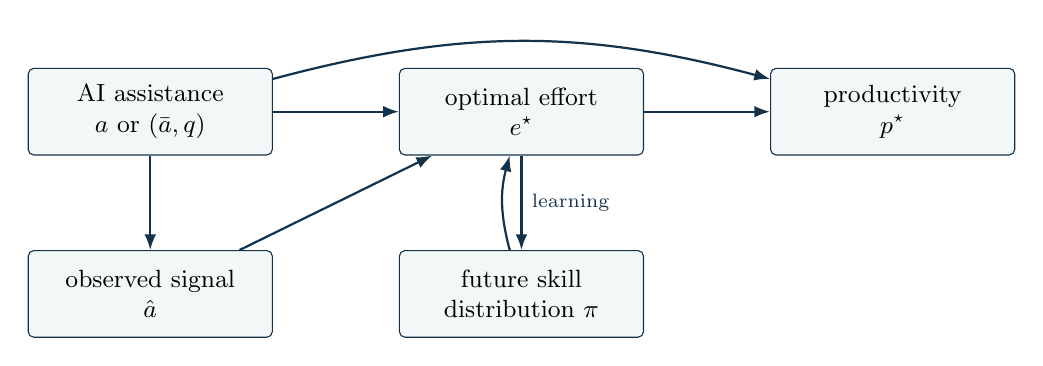
\begin{tikzpicture}[
  node distance=12mm and 16mm,
  box/.style={draw=navy,rounded corners=2pt,fill=pale,minimum width=31mm,
    minimum height=11mm,align=center,font=\small},
  arr/.style={-{Latex[length=2mm]},thick,navy}]
\node[box] (ai) {AI assistance\\$a$ or $(\bar a,q)$};
\node[box,right=of ai] (eff) {optimal effort\\$e^\star$};
\node[box,right=of eff] (prod) {productivity\\$p^\star$};
\node[box,below=of eff] (skill) {future skill\\distribution $\pi$};
\node[box,below=of ai] (signal) {observed signal\\$\hat a$};
\draw[arr] (ai)--(eff);
\draw[arr] (eff)--(prod);
\draw[arr] (ai) to[bend left=15] (prod);
\draw[arr] (eff)--node[right,font=\scriptsize]{learning}(skill);
\draw[arr] (skill) to[bend left=15] (eff);
\draw[arr] (ai)--(signal);
\draw[arr] (signal)--(eff);
\end{tikzpicture}
\vspace{3mm}
\begin{itemize}
  \item \key{Deterministic substitution:} AI replaces effort one for one until effort reaches zero.
  \item \key{Endogenous skill:} lower effort reduces upward skill-transition rates.
  \item \key{Information and reliability:} later sections add random AI and skill-dependent verification.
\end{itemize}
\begin{alertblock}{Scope}
We prove the first two mechanisms completely: tutorial Sections 3 and 4.
\end{alertblock}
\end{frame}

\begin{frame}{Main conclusions before the mathematics}
\begin{enumerate}
  \item \textbf{Exact static optimizer:}
  \[
  e^\star(s,a)=\pos{x^\star-s-a},
  \qquad
  p^\star(s,a)=\max\{p(x^\star),p(s+a)\}.
  \]
  \item \textbf{Skill degradation:} higher AI lowers effort-dependent upward rates, so its stationary skill distribution is first-order stochastically lower.
  \item \textbf{Non-monotone productivity:} within an activity regime, long-run productivity is increasing or increasing-then-decreasing.
  \item \textbf{Sensitivity gap:} for sufficiently rapid skill decay, $\Delta_m>0$ creates a declining region.
  \item \textbf{Composition reversal:} every fixed-skill productivity can rise while the stationary average falls.
\end{enumerate}
\source{Paper Propositions 1 and 3, Theorem 1, and mathematical appendices.}
\end{frame}

\begin{frame}{What students should be able to reconstruct}
\begin{columns}[T,onlytextwidth]
\column{.48\textwidth}
\begin{block}{Static choice}
\begin{itemize}
  \item Change variables from effort to total input.
  \item Derive the positive-part optimizer.
  \item Separate utility from productivity.
  \item Explain the kink at zero effort.
\end{itemize}
\end{block}
\column{.48\textwidth}
\begin{block}{Dynamic skill}
\begin{itemize}
  \item Interpret rates and detailed balance.
  \item Normalize the stationary distribution.
  \item Prove stochastic skill degradation.
  \item Decompose $\calP'(a)$ and prove one crossing.
  \item Recover $\Delta_m$ and the two-state threshold.
\end{itemize}
\end{block}
\end{columns}
\vspace{4mm}
\begin{exampleblock}{Reading rule}
Every result will be obtained from the preceding equations; products, reciprocals, derivatives, and normalizations are unpacked when first used.
\end{exampleblock}
\end{frame}

% ============================================================
% SECTION 3
% ============================================================

\section{Deterministic static choice}

\begin{frame}[plain]
\begin{tikzpicture}[remember picture,overlay]
\fill[navy] (current page.south west) rectangle (current page.north east);
\fill[teal] (current page.south west) rectangle ([xshift=13mm]current page.north west);
\end{tikzpicture}
\vspace{20mm}
{\color{white}\Huge\bfseries Part I\par}
\vspace{4mm}
{\color{white}\LARGE The deterministic basic model\par}
\vspace{8mm}
{\color{white!75}\large Skill and AI set a baseline; effort fills the remaining productive gap.\par}
\end{frame}

\begin{frame}{Three inputs, two economic outcomes}
\begin{columns}[T,onlytextwidth]
\column{.53\textwidth}
\begin{block}{Total productive input}
\[
x=s+e+a
\]
\begin{itemize}
  \item $s\ge0$: current human skill
  \item $e\ge0$: costly human effort
  \item $a\ge0$: deterministic AI assistance
\end{itemize}
\end{block}
\column{.43\textwidth}
\begin{block}{Utility and productivity}
\[
u(e;s,a)=p(s+e+a)-\gamma e
\]
\[
p^\star(s,a)=p(s+e^\star+a)
\]
\end{block}
\end{columns}
\vspace{3mm}
\begin{alertblock}{Do not subtract effort cost from productivity}
The cost $\gamma e$ enters choice and utility, but the paper evaluates gross productive output $p(x)$.
\end{alertblock}
\end{frame}

\begin{frame}{Assumptions make the problem globally tractable}
\begin{itemize}
  \item $p$ is nonnegative, increasing, continuous, differentiable where required, and concave.
  \item Effort has linear cost $c(e)=\gamma e$ with $\gamma>0$.
  \item The agent is myopic: current effort does not internalize future skill.
  \item The maximization problem has a finite largest solution.
\end{itemize}
\vspace{4mm}
Define
\[
g(x):=p(x)-\gamma x.
\]
Because $p$ is concave and $-\gamma x$ is linear, $g$ is concave.
\begin{block}{Largest maximizer}
\[
x^\star:=\max\arg\max_{x\ge0}\{p(x)-\gamma x\}.
\]
The convention makes all later formulas single valued.
\end{block}
\end{frame}

\begin{frame}{Step 1: replace effort by total input}
The original problem is
\[
\max_{e\ge0}\{p(s+e+a)-\gamma e\}.
\]
Set
\[
x=s+e+a
\qquad\Longleftrightarrow\qquad
e=x-s-a.
\]
The constraint $e\ge0$ becomes $x\ge s+a$. Substitution gives
\begin{align*}
p(s+e+a)-\gamma e
&=p(x)-\gamma(x-s-a)\\
&=\underbrace{p(x)-\gamma x}_{g(x)}
+\underbrace{\gamma(s+a)}_{\text{constant in }x}.
\end{align*}
\begin{block}{Equivalent problem}
\[
\max_{x\ge s+a}g(x).
\]
\end{block}
\end{frame}

\begin{frame}{Step 2: identify the preferred total-input target}
Ignoring the lower bound $x\ge s+a$, the agent wants the largest maximizer $x^\star$ of
\[
g(x)=p(x)-\gamma x.
\]
For differentiable $p$, an interior target satisfies
\[
g'(x^\star)=p'(x^\star)-\gamma=0
\quad\Longrightarrow\quad
p'(x^\star)=\gamma.
\]
Concavity implies
\[
p'(x)>\gamma\quad(x<x^\star),
\qquad
p'(x)<\gamma\quad(x>x^\star),
\]
with weak inequalities when $p$ has flat portions.
\begin{exampleblock}{Economic reading}
$x^\star$ equates marginal production to the marginal cost of generating input through effort.
\end{exampleblock}
\end{frame}

\begin{frame}{Step 3: impose the feasible lower bound}
The feasible set is the half-line $[s+a,\infty)$.
\begin{columns}[T,onlytextwidth]
\column{.48\textwidth}
\begin{block}{Target remains feasible}
If $s+a\le x^\star$, then $x^\star$ is feasible:
\[
x^{\mathrm{opt}}=x^\star.
\]
\end{block}
\column{.48\textwidth}
\begin{alertblock}{Baseline exceeds target}
If $s+a>x^\star$, the agent cannot reduce total input. Concavity makes $g$ decrease to the right:
\[
x^{\mathrm{opt}}=s+a.
\]
\end{alertblock}
\end{columns}
\vspace{4mm}
\[
\boxed{x^{\mathrm{opt}}=\max\{x^\star,s+a\}.}
\]
\end{frame}

\begin{frame}{Case 1: effort fills the gap exactly}
Suppose $s+a\le x^\star$. The target is feasible, so
\[
e^\star=x^\star-s-a\ge0.
\]
Then
\[
s+e^\star+a
=s+(x^\star-s-a)+a
=x^\star.
\]
\begin{block}{One-for-one substitution}
While effort is positive,
\[
\frac{\partial e^\star}{\partial a}=-1.
\]
One more unit of AI reduces effort by one unit; total input and productivity remain unchanged.
\end{block}
\end{frame}

\begin{frame}{Case 2: effort cannot be negative}
Suppose $s+a>x^\star$. Reaching the target would require
\[
e=x^\star-s-a<0,
\]
which violates $e\ge0$.
\vspace{2mm}
Any positive effort would push total input farther to the right, where concavity makes $g$ weakly decreasing. Therefore
\[
e^\star=0,
\qquad
x^{\mathrm{opt}}=s+a.
\]
\begin{alertblock}{The corner is economically meaningful}
Once skill plus AI exceeds the target, effort is exhausted and further AI raises total input directly.
\end{alertblock}
\end{frame}

\begin{frame}{Step 4: combine both cases with the positive part}
For any real number $z$, define
\[
z_+:=\max\{z,0\}
=
\begin{cases}
z,&z\ge0,\\
0,&z<0.
\end{cases}
\]
The two effort cases become
\[
\boxed{e^\star(s,a)=\pos{x^\star-s-a}.}
\]
Equivalently,
\[
e^\star(s,a)=
\begin{cases}
x^\star-s-a,&s+a\le x^\star,\\
0,&s+a>x^\star.
\end{cases}
\]
\begin{exampleblock}{Notation checkpoint}
The subscript $+$ applies to the entire expression. It is not an additional positive term.
\end{exampleblock}
\end{frame}

\begin{frame}{Step 5: evaluate productivity at optimal input}
Productivity excludes effort cost:
\[
p^\star(s,a)=p(s+e^\star(s,a)+a).
\]
From the optimal total input,
\[
s+e^\star+a=\max\{x^\star,s+a\}.
\]
Therefore
\begin{align*}
p^\star(s,a)
&=p\!\left(\max\{x^\star,s+a\}\right)\\
&=\max\{p(x^\star),p(s+a)\},
\end{align*}
because $p$ is increasing.
\[
\boxed{p^\star(s,a)=\max\{p(x^\star),p(s+a)\}.}
\]
\end{frame}

\begin{frame}{The deterministic optimizer has a kink}
\[
\frac{\partial e^\star}{\partial a}
=
\begin{cases}
-1,&a<x^\star-s,\\
0,&a>x^\star-s,
\end{cases}
\]
\[
\frac{\partial p^\star}{\partial a}
=
\begin{cases}
0,&a<x^\star-s,\\
p'(s+a)\ge0,&a>x^\star-s.
\end{cases}
\]
\begin{block}{Two phases}
\key{Replacement phase:} AI crowds out effort with no output gain.\\[1mm]
\key{Expansion phase:} effort is zero and AI raises output directly.
\end{block}
\vspace{2mm}
At $a=x^\star-s$, the level is continuous but the derivative formula changes.
\end{frame}

\begin{frame}{Worked example: logarithmic production}
Let
\[
p(x)=\alpha\log(1+x),
\qquad 0<\gamma<\alpha.
\]
The first-order condition is
\[
\frac{\alpha}{1+x}=\gamma
\quad\Longrightarrow\quad
x^\star=\frac{\alpha}{\gamma}-1.
\]
Hence
\[
e^\star(s,a)=
\pos{\frac{\alpha}{\gamma}-1-s-a},
\]
\[
p^\star(s,a)=
\alpha\log\!\left(
1+\max\left\{\frac{\alpha}{\gamma}-1,s+a\right\}
\right).
\]
\begin{exampleblock}{Threshold}
Effort reaches zero at $a=x^\star-s=\alpha/\gamma-1-s$.
\end{exampleblock}
\end{frame}

\begin{frame}{Numerical reading of the positive part}
Suppose $x^\star=5$.
\begin{columns}[T,onlytextwidth]
\column{.48\textwidth}
\begin{block}{$s=2$, $a=1$}
\[
s+a=3<5,
\qquad
e^\star=(5-2-1)_+=2.
\]
Total input:
\[
2+2+1=5=x^\star.
\]
\end{block}
\column{.48\textwidth}
\begin{alertblock}{$s=4$, $a=2$}
\[
s+a=6>5.
\]
The raw expression is $-1$, so
\[
e^\star=(-1)_+=0.
\]
Total input is $6$.
\end{alertblock}
\end{columns}
\end{frame}

\begin{frame}{Section 3 checkpoint}
\begin{enumerate}
  \item Changing variables reveals that the real target is total input.
  \item $x^\star$ solves the unconstrained concave problem.
  \item Skill plus AI is a baseline that cannot be undone.
  \item Effort fills the missing gap when the baseline is below $x^\star$.
  \item Once the baseline reaches $x^\star$, effort is zero and further AI raises productivity.
\end{enumerate}
\vspace{3mm}
\begin{alertblock}{The dynamic question}
If effort is also the input into learning, what happens to future skill when AI replaces current effort?
\end{alertblock}
\end{frame}

% ============================================================
% SECTION 4
% ============================================================

\section{Endogenous skill development}

\begin{frame}[plain]
\begin{tikzpicture}[remember picture,overlay]
\fill[navy] (current page.south west) rectangle (current page.north east);
\fill[gold] (current page.south west) rectangle ([xshift=13mm]current page.north west);
\end{tikzpicture}
\vspace{20mm}
{\color{white}\Huge\bfseries Part II\par}
\vspace{4mm}
{\color{white}\LARGE Endogenous skill and the first paradox\par}
\vspace{8mm}
{\color{white!75}\large Current effort determines how quickly the agent moves toward higher skill.\par}
\end{frame}

\begin{frame}{The feedback loop changes the static conclusion}
At skill state $s_k$, optimal effort is
\[
e_k(a):=e^\star(s_k,a)=\pos{x^\star-s_k-a}.
\]
Effort controls the upward transition rate:
\[
s_k\longrightarrow s_{k+1}
\quad\text{at rate}\quad
\lambda(e_k(a)).
\]
Skill depreciates at constant rate:
\[
s_k\longrightarrow s_{k-1}
\quad\text{at rate}\quad
\mu>0.
\]
\begin{align*}
a\uparrow
&\Rightarrow e_k(a)\downarrow
\Rightarrow\lambda(e_k(a))\downarrow\\
&\Rightarrow\text{less stationary mass on high skill}\\
&\Rightarrow\text{possible decline in long-run productivity.}
\end{align*}
\end{frame}

\begin{frame}{What is a transition rate?}
The model runs in continuous time. A rate describes how quickly events arrive; it is \emph{not} itself a probability.
\vspace{2mm}
If the process is at $s_i$ and the rate of moving to $s_j$ is $r_{ij}$, then for a short interval of length $h$,
\[
\Pp(S(t+h)=s_j\mid S(t)=s_i)
=r_{ij}h+o(h),
\qquad i\ne j.
\]
The notation $o(h)$ means
\[
\frac{o(h)}{h}\longrightarrow0
\quad\text{as }h\downarrow0.
\]
\begin{alertblock}{Units matter}
A rate may exceed one because it is measured per unit of time. The short-interval probability is approximately rate $\times$ interval length.
\end{alertblock}
\end{frame}

\begin{frame}{Short-interval probabilities at an interior state}
Write
\[
\lambda_k(a):=\lambda(e_k(a)).
\]
Conditional on being at an interior state $s_k$,
\begin{align*}
\Pp(\text{move up in }[t,t+h])
&=\lambda_k(a)h+o(h),\\
\Pp(\text{move down in }[t,t+h])
&=\mu h+o(h),\\
\Pp(\text{remain at }s_k)
&=1-[\lambda_k(a)+\mu]h+o(h).
\end{align*}
The probability of two or more moves is $o(h)$.
\begin{block}{Boundary states}
At $s_1$ there is no downward move. At $s_N$ there is no upward move.
\end{block}
\end{frame}

\begin{frame}{Competing clocks turn rates into probabilities}
At an interior state, the upward and downward moves act like exponential clocks:
\[
\text{total event rate}=\lambda_k+\mu.
\]
Therefore
\[
\E[\text{waiting time to next change}]
=\frac{1}{\lambda_k+\mu},
\]
\[
\Pp(\text{up next})
=\frac{\lambda_k}{\lambda_k+\mu},
\qquad
\Pp(\text{down next})
=\frac{\mu}{\lambda_k+\mu}.
\]
\begin{exampleblock}{Example}
If $\lambda_k=0.30$ per year and $\mu=0.10$ per year, the expected wait is $2.5$ years and the next change is upward with probability $0.75$.
\end{exampleblock}
\end{frame}

\begin{frame}{The skill process is a birth--death chain}
\centering
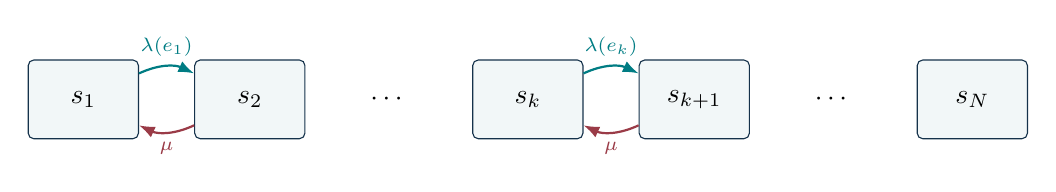
\begin{tikzpicture}[
  node distance=7mm,
  state/.style={draw=navy,rounded corners=2pt,fill=pale,minimum width=14mm,
    minimum height=10mm,align=center},
  up/.style={-{Latex[length=2mm]},bend left=25,thick,teal},
  down/.style={-{Latex[length=2mm]},bend left=25,thick,rose}]
\node[state] (s1) {$s_1$};
\node[state,right=of s1] (s2) {$s_2$};
\node[right=of s2] (dots) {$\cdots$};
\node[state,right=of dots] (sk) {$s_k$};
\node[state,right=of sk] (skp) {$s_{k+1}$};
\node[right=of skp] (dots2) {$\cdots$};
\node[state,right=of dots2] (sn) {$s_N$};
\draw[up] (s1) to node[above,font=\scriptsize] {$\lambda(e_1)$} (s2);
\draw[down] (s2) to node[below,font=\scriptsize] {$\mu$} (s1);
\draw[up] (sk) to node[above,font=\scriptsize] {$\lambda(e_k)$} (skp);
\draw[down] (skp) to node[below,font=\scriptsize] {$\mu$} (sk);
\end{tikzpicture}
\vspace{5mm}
\begin{itemize}
  \item Only neighboring moves are allowed.
  \item $\lambda(e)>0$, $\lambda'(e)\ge0$, and $\lambda''(e)\le0$.
  \item More effort speeds learning, but its marginal effect is diminishing.
\end{itemize}
\end{frame}

\begin{frame}{The generator records instantaneous rates}
For $k=2,\ldots,N-1$, the generator matrix $Q$ has
\[
Q_{k,k+1}=\lambda_k,
\qquad
Q_{k,k-1}=\mu,
\qquad
Q_{k,k}=-(\lambda_k+\mu).
\]
All other entries in row $k$ are zero, so
\[
\sum_jQ_{k,j}=0.
\]
\begin{alertblock}{The diagonal is not a negative probability}
$Q_{k,k}$ is a bookkeeping term representing total outflow. The stationary condition is
\[
\pi Q=0.
\]
\end{alertblock}
\end{frame}

\begin{frame}{Stationarity is a long-run time allocation}
Fix the AI level $a$. Define
\[
\pi_k(a):=\text{long-run probability of skill state }s_k.
\]
Equivalently, $\pi_k(a)$ is the long-run fraction of time spent at $s_k$.
\[
\pi_k(a)\ge0,
\qquad
\sum_{k=1}^N\pi_k(a)=1.
\]
\begin{block}{Stationarity}
The distribution does not change over time. At each state,
\[
\text{probability inflow per unit time}
=
\text{probability outflow per unit time}.
\]
\end{block}
\end{frame}

\begin{frame}{Detailed balance equates flow across one edge}
Consider the edge connecting $s_k$ and $s_{k+1}$.
\begin{itemize}
  \item Mass at $s_k$ is $\pi_k(a)$ and moves upward at rate $\lambda_k(a)$:
  \[
  \text{upward flow}=\pi_k(a)\lambda_k(a).
  \]
  \item Mass at $s_{k+1}$ is $\pi_{k+1}(a)$ and moves downward at rate $\mu$:
  \[
  \text{downward flow}=\pi_{k+1}(a)\mu.
  \]
\end{itemize}
Detailed balance sets the opposite flows equal:
\[
\boxed{\pi_k(a)\lambda_k(a)=\pi_{k+1}(a)\mu.}
\]
Both sides have units of probability mass per unit of time.
\end{frame}

\begin{frame}{Detailed balance gives an adjacent recursion}
Because $\mu>0$, divide by $\mu$:
\[
\boxed{
\pi_{k+1}(a)=\pi_k(a)\frac{\lambda_k(a)}{\mu}.}
\]
Divide once more by $\pi_k(a)>0$:
\[
\boxed{
\frac{\pi_{k+1}(a)}{\pi_k(a)}
=\frac{\lambda_k(a)}{\mu}.}
\]
\begin{itemize}
  \item If $\lambda_k>\mu$, stationary mass rises from $s_k$ to $s_{k+1}$.
  \item If $\lambda_k<\mu$, stationary mass falls.
  \item If $\lambda_k=\mu$, the neighboring probabilities are equal.
\end{itemize}
\end{frame}

\begin{frame}{Repeated substitution produces the product formula}
\begin{align*}
\pi_2(a)
&=\pi_1(a)\frac{\lambda_1(a)}{\mu},\\
\pi_3(a)
&=\pi_2(a)\frac{\lambda_2(a)}{\mu}
=\pi_1(a)\frac{\lambda_1(a)}{\mu}
\frac{\lambda_2(a)}{\mu},\\
\pi_4(a)
&=\pi_1(a)\frac{\lambda_1(a)}{\mu}
\frac{\lambda_2(a)}{\mu}
\frac{\lambda_3(a)}{\mu}.
\end{align*}
Hence
\[
\boxed{
\pi_k(a)=\pi_1(a)
\prod_{i=1}^{k-1}
\frac{\lambda(e_i(a))}{\mu}.}
\]
Each factor corresponds to one intervening edge.
\end{frame}

\begin{frame}{How to read the product symbol}
\[
\prod_{i=1}^{k-1}\frac{\lambda_i(a)}{\mu}
=
\frac{\lambda_1(a)}{\mu}
\frac{\lambda_2(a)}{\mu}
\cdots
\frac{\lambda_{k-1}(a)}{\mu}.
\]
It multiplies the upward-to-downward rate ratio on every edge between $s_1$ and $s_k$.
\vspace{3mm}
For $k=1$, there are no factors:
\[
\prod_{i=1}^{0}\frac{\lambda_i(a)}{\mu}=1.
\]
\begin{exampleblock}{Empty-product convention}
The value one makes the general formula work at $k=1$:
\[
\pi_1(a)=\pi_1(a)\times1.
\]
\end{exampleblock}
\end{frame}

\begin{frame}{Normalization determines the remaining constant}
\begin{align*}
1
&=\sum_{k=1}^N\pi_k(a)\\
&=\pi_1(a)+
\sum_{k=2}^N
\pi_1(a)\prod_{i=1}^{k-1}
\frac{\lambda(e_i(a))}{\mu}\\
&=\pi_1(a)\left[
1+\sum_{k=2}^N
\prod_{i=1}^{k-1}
\frac{\lambda(e_i(a))}{\mu}
\right].
\end{align*}
Therefore
\[
\boxed{
\pi_1(a)=
\left[
1+\sum_{k=2}^N
\prod_{i=1}^{k-1}
\frac{\lambda(e_i(a))}{\mu}
\right]^{-1}.}
\]
\end{frame}

\begin{frame}{Why the exponent \texorpdfstring{$-1$}{-1} appears}
Let
\[
Z(a):=
1+\sum_{k=2}^N
\prod_{i=1}^{k-1}\frac{\lambda(e_i(a))}{\mu}.
\]
Normalization gave
\[
1=\pi_1(a)Z(a).
\]
Divide by $Z(a)>0$:
\[
\pi_1(a)=\frac{1}{Z(a)}=Z(a)^{-1}.
\]
\begin{block}{Interpretation}
$Z(a)$ is the normalization constant. Its reciprocal rescales the positive weights so that the probabilities sum to one.
\end{block}
\end{frame}

\begin{frame}{Stationary outcomes are weighted averages}
At state $s_k$:
\[
\text{effort}=e_k(a),
\qquad
\text{productivity}=p^\star(s_k,a).
\]
The law of total expectation gives
\[
\boxed{
\calE(a)=\sum_{k=1}^N\pi_k(a)e_k(a),}
\]
\[
\boxed{
\calP(a)=\sum_{k=1}^N
\pi_k(a)p^\star(s_k,a).}
\]
\begin{exampleblock}{Reading the formula}
Each state-specific outcome is multiplied by the long-run fraction of time spent in that state.
\end{exampleblock}
\end{frame}

\begin{frame}{Two-state stationary example}
Suppose
\[
\lambda_1=0.30,
\qquad
\mu=0.10.
\]
Detailed balance gives
\[
\pi_1(0.30)=\pi_2(0.10)
\quad\Longrightarrow\quad
\pi_2=3\pi_1.
\]
Together with $\pi_1+\pi_2=1$:
\[
\pi_1=0.25,\qquad\pi_2=0.75.
\]
If efforts are $(2,0.5)$ and productivities are $(10,16)$:
\[
\calE=0.25(2)+0.75(0.5)=0.875,
\qquad
\calP=0.25(10)+0.75(16)=14.5.
\]
\end{frame}

\begin{frame}{Edge balance solves full stationarity}
At an interior state $s_k$,
\[
\pi_{k-1}\lambda_{k-1}
+\pi_{k+1}\mu
-\pi_k(\lambda_k+\mu)=0.
\]
Detailed balance on the lower and upper edges gives
\[
\pi_{k-1}\lambda_{k-1}=\pi_k\mu,
\qquad
\pi_{k+1}\mu=\pi_k\lambda_k.
\]
Substitute:
\begin{align*}
\pi_{k-1}\lambda_{k-1}
+\pi_{k+1}\mu
-\pi_k(\lambda_k+\mu)
&=\pi_k\mu+\pi_k\lambda_k
-\pi_k(\lambda_k+\mu)\\
&=0.
\end{align*}
The boundary equations are the first and last detailed-balance equations.
\end{frame}

\begin{frame}{Activity is determined by a state threshold}
Recall
\[
e_k(a)=\pos{x^\star-s_k-a}.
\]
Then
\begin{align*}
e_k(a)>0
&\Longleftrightarrow x^\star-s_k-a>0\\
&\Longleftrightarrow a<x^\star-s_k\\
&\Longleftrightarrow s_k+a<x^\star.
\end{align*}
Because $s_1\le\cdots\le s_N$,
\[
x^\star-s_1\ge\cdots\ge x^\star-s_N.
\]
\begin{block}{Ordering implication}
High-skill states stop exerting effort first. Active states always form a lower block $\{1,\ldots,m\}$.
\end{block}
\end{frame}

\begin{frame}{Constructing the activity interval \texorpdfstring{$I_m$}{Im}}
If exactly the first $m$ states are active in the interior, then
\[
a<x^\star-s_m,
\qquad
a\ge x^\star-s_{m+1}.
\]
The paper defines
\[
I_m=
\left(
\pos{x^\star-s_{m+1}},
\pos{x^\star-s_m}
\right],
\quad m=1,\ldots,N-1,
\]
with
\[
I_0=[\pos{x^\star-s_1},\infty),
\qquad
I_N=[0,\pos{x^\star-s_N}].
\]
\begin{exampleblock}{Meaning}
$I_m$ is the regime with $m$ active states away from shared endpoints.
\end{exampleblock}
\end{frame}

\begin{frame}{Within one regime, all formulas are smooth}
For $a$ in the interior of $I_m$:
\[
\begin{array}{lll}
k\le m:
&e_k=x^\star-s_k-a>0,
&p_k^\star=p(x^\star),\\[1mm]
k\ge m+1:
&e_k=0,
&p_k^\star=p(s_k+a).
\end{array}
\]
Therefore
\[
e_k'(a)=
\begin{cases}
-1,&k\le m,\\
0,&k\ge m+1,
\end{cases}
\quad
\frac{d}{da}p_k^\star(a)=
\begin{cases}
0,&k\le m,\\
p'(s_k+a),&k\ge m+1.
\end{cases}
\]
Only at a regime boundary does one state change formula.
\end{frame}

\begin{frame}{Example: locate all activity regimes}
Let
\[
x^\star=10,
\qquad
(s_1,s_2,s_3)=(2,6,9).
\]
The thresholds are
\[
x^\star-s_1=8,
\qquad
x^\star-s_2=4,
\qquad
x^\star-s_3=1.
\]
Hence
\[
I_3=[0,1],\quad
I_2=(1,4],\quad
I_1=(4,8],\quad
I_0=[8,\infty).
\]
At $a=3\in I_2$:
\[
e_1=5,\qquad e_2=1,\qquad e_3=0.
\]
\end{frame}

\begin{frame}{The sensitivity gap compares two responses}
Fix an intermediate regime and define
\[
a_m:=x^\star-s_m,
\qquad
d_m:=s_{m+1}-s_m>0.
\]
At $a=a_m$, for every active $j\le m$,
\[
e_j(a_m)
=x^\star-s_j-(x^\star-s_m)
=s_m-s_j.
\]
The first inactive state has total input
\[
s_{m+1}+a_m
=x^\star+s_{m+1}-s_m
=x^\star+d_m.
\]
\begin{block}{Why these substitutions matter}
They explain every argument appearing in $\Delta_m$.
\end{block}
\end{frame}

\begin{frame}{A semi-elasticity is a logarithmic derivative}
For any positive differentiable function $f$,
\[
\frac{f'(x)}{f(x)}
=\frac{d}{dx}\log f(x).
\]
It measures the proportional change in $f$ caused by a one-unit change in $x$.
\vspace{3mm}
For the reciprocal active-rate product
\[
A_{1,m}(a)=
\left[
\prod_{j=1}^{m}
\lambda(x^\star-s_j-a)
\right]^{-1},
\]
take logarithms:
\[
\log A_{1,m}(a)
=-\sum_{j=1}^m
\log\lambda(x^\star-s_j-a).
\]
\end{frame}

\begin{frame}{Differentiate the learning sensitivity}
Differentiate
\[
\log A_{1,m}(a)
=-\sum_{j=1}^m
\log\lambda(x^\star-s_j-a).
\]
The derivative of $x^\star-s_j-a$ is $-1$, canceling the outer minus sign:
\begin{align*}
\frac{A_{1,m}'(a)}{A_{1,m}(a)}
&=\frac{d}{da}\log A_{1,m}(a)\\
&=\sum_{j=1}^m
\frac{\lambda'(x^\star-s_j-a)}
{\lambda(x^\star-s_j-a)}.
\end{align*}
At $a=a_m$,
\[
\frac{A_{1,m}'(a_m)}{A_{1,m}(a_m)}
=
\sum_{j=1}^m
\frac{\lambda'(s_m-s_j)}
{\lambda(s_m-s_j)}.
\]
\end{frame}

\begin{frame}{The direct channel is a productivity premium}
Define the premium of the first inactive state:
\[
R_m(a):=
p(s_{m+1}+a)-p(x^\star)>0.
\]
Because $p(x^\star)$ is constant,
\[
R_m'(a)=p'(s_{m+1}+a).
\]
Therefore
\[
\frac{R_m'(a)}{R_m(a)}
=
\frac{p'(s_{m+1}+a)}
{p(s_{m+1}+a)-p(x^\star)}.
\]
At $a=a_m$,
\[
\frac{R_m'(a_m)}{R_m(a_m)}
=
\frac{p'(x^\star+d_m)}
{p(x^\star+d_m)-p(x^\star)}.
\]
\end{frame}

\begin{frame}{Learning sensitivity minus productivity sensitivity}
\[
\boxed{
\Delta_m=
\underbrace{
\sum_{j=1}^m
\frac{\lambda'(s_m-s_j)}
{\lambda(s_m-s_j)}
}_{\text{learning-weight sensitivity}}
-
\underbrace{
\frac{p'(x^\star+d_m)}
{p(x^\star+d_m)-p(x^\star)}
}_{\text{productivity-premium sensitivity}}.}
\]
\begin{itemize}
  \item $\Delta_m>0$: the deskilling channel is locally more sensitive.
  \item $\Delta_m<0$: the direct productivity channel is locally more sensitive.
\end{itemize}
\begin{alertblock}{Clarification}
The sign of $\Delta_m$ alone does not determine $\calP'(a)$ for every $\mu$. Decay controls how strongly these sensitivities enter stationary weights.
\end{alertblock}
\end{frame}

\begin{frame}{Numerical reading of \texorpdfstring{$\Delta_1$}{Delta1}}
Take
\[
\lambda(e)=1+e,\quad
p(x)=\log(1+x),\quad
x^\star=3,\quad s_1=0,\quad s_2=2.
\]
Then $d_1=2$ and
\[
\frac{\lambda'(0)}{\lambda(0)}=1.
\]
The productivity-premium sensitivity is
\[
\frac{p'(5)}{p(5)-p(3)}
=
\frac{1/6}{\log(6)-\log(4)}
\approx0.411.
\]
Hence
\[
\Delta_1\approx1-0.411=0.589>0.
\]
The learning channel is locally more sensitive.
\end{frame}

\begin{frame}{First-order stochastic dominance: the target}
Let $a_\ell<a_h$. Lower AI should produce a higher skill distribution.
\vspace{3mm}
Define the lower-tail probability
\[
F^q(k):=\sum_{j=1}^k\pi_j(a_q),
\qquad q\in\{\ell,h\}.
\]
The low-AI distribution first-order stochastically dominates the high-AI distribution if
\[
\boxed{
F^\ell(k)\le F^h(k)
\quad\text{for every }k.}
\]
\begin{block}{Why the inequality points this way}
A smaller probability of being among the lowest $k$ states means more probability on higher skill states.
\end{block}
\end{frame}

\begin{frame}{Step 1: compare every adjacent ratio}
The deterministic optimizer implies
\[
e_i(a_\ell)\ge e_i(a_h)
\qquad\text{for every }i.
\]
Since $\lambda$ is increasing and $\mu$ is unchanged,
\[
r_i^\ell:=
\frac{\lambda(e_i(a_\ell))}{\mu}
\ge
r_i^h:=
\frac{\lambda(e_i(a_h))}{\mu}.
\]
Detailed balance gave
\[
r_i^q=\frac{\pi_{i+1}(a_q)}{\pi_i(a_q)}.
\]
\begin{exampleblock}{Meaning}
Every adjacent high-to-low probability ratio is more favorable to high skill under lower AI.
\end{exampleblock}
\end{frame}

\begin{frame}{Step 2: remove normalization}
Define unnormalized weights
\[
w_1^q=1,
\qquad
w_k^q=\prod_{i=1}^{k-1}r_i^q
\quad(k\ge2),
\]
and
\[
T^q=\sum_{j=1}^Nw_j^q.
\]
Then
\[
\pi_k(a_q)=\frac{w_k^q}{T^q},
\qquad
F^q(k)=
\frac{\sum_{j=1}^k w_j^q}
{\sum_{j=1}^N w_j^q}.
\]
The problem is now a comparison between normalized products of ordered adjacent ratios.
\end{frame}

\begin{frame}{Step 3: cross-multiply positive denominators}
\small
Because all weights are positive,
\begin{align*}
F^\ell(k)\le F^h(k)
\Longleftrightarrow
\left(\sum_{j=1}^k w_j^\ell\right)
\left(\sum_{n=1}^N w_n^h\right)
\le
\left(\sum_{j=1}^k w_j^h\right)
\left(\sum_{n=1}^N w_n^\ell\right).
\end{align*}
After expansion, terms with both $j\le k$ and $n\le k$ cancel after interchanging the dummy indices.
\vspace{3mm}
It remains to prove, for every cross-block pair $j\le k<n$,
\[
\boxed{
w_j^\ell w_n^h
\le
w_j^h w_n^\ell.}
\]
\end{frame}

\begin{frame}{Step 4: prove each cross-block comparison}
Since $n>j$, all factors before edge $j$ cancel:
\begin{align*}
\frac{w_n^\ell}{w_j^\ell}
&=
\frac{\prod_{i=1}^{n-1}r_i^\ell}
{\prod_{i=1}^{j-1}r_i^\ell}\\
&=
\prod_{i=j}^{n-1}r_i^\ell
\ge
\prod_{i=j}^{n-1}r_i^h
=
\frac{w_n^h}{w_j^h}.
\end{align*}
Multiplying by $w_j^\ell w_j^h>0$ gives
\[
w_j^\ell w_n^h\le w_j^h w_n^\ell.
\]
Summing over all cross-block pairs proves
\[
F^\ell(k)\le F^h(k).
\]
\end{frame}

\begin{frame}{Skill degradation proposition}
\begin{block}{Proposition}
For $a_\ell<a_h$,
\[
\boxed{
\sum_{i=1}^k\pi_i(a_\ell)
\le
\sum_{i=1}^k\pi_i(a_h),
\qquad k=1,\ldots,N.}
\]
\end{block}
\vspace{3mm}
\begin{center}
\large More AI lowers effort, lowers every upward rate, and shifts long-run mass toward low skill.
\end{center}
\vspace{3mm}
\begin{alertblock}{What remains}
The proposition establishes a downward skill shift, but aggregate productivity also has a positive direct AI effect. We still need to compare magnitudes.
\end{alertblock}
\end{frame}

\begin{frame}{Three-state dominance example}
Suppose
\[
(r_1^\ell,r_2^\ell)=(2,1.5),
\qquad
(r_1^h,r_2^h)=(1,0.75).
\]
The unnormalized weights are
\[
w^\ell=(1,2,3),
\qquad
w^h=(1,1,0.75).
\]
After normalization,
\[
\pi(a_\ell)=
\left(\frac16,\frac13,\frac12\right),
\qquad
\pi(a_h)=
\left(\frac4{11},\frac4{11},\frac3{11}\right).
\]
Lower tails:
\[
\frac16<\frac4{11},
\qquad
\frac12<\frac8{11}.
\]
\end{frame}

\begin{frame}{Rewrite productivity using unnormalized weights}
Fix an intermediate regime $I_m$. Define
\[
q_1(a)=1,
\qquad
q_k(a)=
\prod_{i=1}^{k-1}
\frac{\lambda(e_i(a))}{\mu}.
\]
Then
\[
\pi_k(a)=
\frac{q_k(a)}
{\sum_{j=1}^Nq_j(a)}.
\]
Therefore
\[
\boxed{
\calP(a)=
\frac{
\sum_{k=1}^Nq_k(a)p_k^\star(a)}
{\sum_{k=1}^Nq_k(a)}.}
\]
The common stationary normalization constant has canceled.
\end{frame}

\begin{frame}{Split active and inactive weights}
Inside $I_m$,
\[
\lambda(e_i(a))=
\begin{cases}
\lambda(x^\star-s_i-a),&i\le m,\\
\lambda(0),&i\ge m+1.
\end{cases}
\]
For $k\le m$,
\[
q_k(a)=
\frac{
\prod_{i=1}^{k-1}
\lambda(x^\star-s_i-a)}
{\mu^{k-1}}.
\]
For $k\ge m+1$,
\[
q_k(a)=
\frac{
\left[\prod_{i=1}^{m}
\lambda(x^\star-s_i-a)\right]
\lambda(0)^{k-m-1}}
{\mu^{k-1}}.
\]
\end{frame}

\begin{frame}{Subtract the common active-state productivity}
Let $Q(a)=\sum_kq_k(a)$. Active states produce $p(x^\star)$:
\begin{align*}
\calP(a)
&=
\frac{
p(x^\star)\sum_{k=1}^mq_k
+\sum_{k=m+1}^Nq_kp(s_k+a)}
{Q(a)}\\
&=
\frac{
p(x^\star)Q(a)
+\sum_{k=m+1}^Nq_k
[p(s_k+a)-p(x^\star)]}
{Q(a)}\\
&=
p(x^\star)
+
\frac{
\sum_{k=m+1}^Nq_k
[p(s_k+a)-p(x^\star)]}
{Q(a)}.
\end{align*}
\end{frame}

\begin{frame}{Cancel the common active-rate product}
Define
\[
C_m(a):=
\prod_{i=1}^m
\lambda(x^\star-s_i-a)>0.
\]
For $k\le m$,
\begin{align*}
\frac{q_k(a)}{C_m(a)}
&=
\frac{
\prod_{i=1}^{k-1}\lambda(x^\star-s_i-a)}
{\mu^{k-1}
\prod_{i=1}^{m}\lambda(x^\star-s_i-a)}\\
&=
\frac{1}{
\mu^{k-1}
\prod_{i=k}^{m}\lambda(x^\star-s_i-a)}.
\end{align*}
For $k\ge m+1$,
\[
\frac{q_k(a)}{C_m(a)}
=
\frac{\lambda(0)^{k-m-1}}{\mu^{k-1}}.
\]
\end{frame}

\begin{frame}{Define the active and inactive blocks}
\small
\[
A_{k,m}(a):=
\left[
\prod_{i=k}^{m}
\lambda(x^\star-s_i-a)
\right]^{-1},
\qquad
B_{k,m}:=\lambda(0)^{k-m-1}.
\]
Then
\[
\boxed{
\calP(a)=p(x^\star)+
\frac{N_m(a)}{D_m(a)},}
\]
where
\[
N_m(a)=
\sum_{k=m+1}^{N}
\frac{B_{k,m}}{\mu^{k-1}}
[p(s_k+a)-p(x^\star)],
\]
\[
D_m(a)=
\sum_{k=1}^{m}
\frac{A_{k,m}(a)}{\mu^{k-1}}
+
\sum_{k=m+1}^{N}
\frac{B_{k,m}}{\mu^{k-1}}>0.
\]
\end{frame}

\begin{frame}{Differentiate every component}
The $B_{k,m}$ are constant in $a$, so
\[
N_m'(a)=
\sum_{k=m+1}^N
\frac{B_{k,m}}{\mu^{k-1}}
p'(s_k+a).
\]
Only active terms in $D_m$ vary:
\[
D_m'(a)=
\sum_{k=1}^m
\frac{A_{k,m}'(a)}{\mu^{k-1}}.
\]
Logarithmic differentiation gives
\[
A_{k,m}'(a)=A_{k,m}(a)L_{k,m}(a),
\]
\[
L_{k,m}(a)=
\sum_{j=k}^m
\frac{\lambda'(x^\star-s_j-a)}
{\lambda(x^\star-s_j-a)}\ge0.
\]
\end{frame}

\begin{frame}{The quotient rule separates gain and loss}
\small
\begin{align*}
\calP'(a)=\frac{1}{D_m(a)^2}
\Bigg[
&
\left(
\sum_{k=m+1}^N
\frac{B_{k,m}}{\mu^{k-1}}
p'(s_k+a)
\right)D_m(a)\\
&-
N_m(a)
\left(
\sum_{k=1}^m
\frac{A_{k,m}'(a)}{\mu^{k-1}}
\right)
\Bigg].
\end{align*}
\begin{itemize}
  \item First term: direct productivity gains in inactive states.
  \item Second term: loss caused by endogenous changes in stationary weights.
\end{itemize}
Since $D_m(a)^2>0$, only the bracket determines the sign.
\end{frame}

\begin{frame}{Rewrite the sign as benefit minus loss}
Define
\[
U_m(a):=
\sum_{k=m+1}^N
\frac{B_{k,m}}{\mu^{k-1}}p'(s_k+a),
\]
\[
V_m(a):=
\sum_{k=m+1}^N
\frac{B_{k,m}}{\mu^{k-1}}
[p(s_k+a)-p(x^\star)],
\]
\[
h_m(a):=\frac{D_m'(a)}{D_m(a)}.
\]
Multiplying the derivative by $D_m>0$ gives
\[
\boxed{
D_m(a)\calP'(a)
=U_m(a)-V_m(a)h_m(a)
=:G_m(a).}
\]
$G_m$ and $\calP'$ always have the same sign.
\end{frame}

\begin{frame}{Two monotonicities are immediate}
\begin{block}{Direct marginal benefit falls}
Concavity of $p$ makes $p'$ weakly decreasing. Positive constant weights imply
\[
U_m(a)\ \text{is weakly decreasing}.
\]
\end{block}
\begin{block}{The productivity premium rises}
Monotonicity of $p$ makes each
\[
p(s_k+a)-p(x^\star)
\]
weakly increasing, so
\[
V_m(a)\ \text{is weakly increasing}.
\]
\end{block}
It remains to show that
\[
h_m(a)=D_m'(a)/D_m(a)
\]
is weakly increasing.
\end{frame}

\begin{frame}{Rewrite \texorpdfstring{$h_m$}{hm} compactly}
Put
\[
\bar A_k(a):=
\frac{A_{k,m}(a)}{\mu^{k-1}},
\qquad
\bar B:=
\sum_{k=m+1}^N
\frac{B_{k,m}}{\mu^{k-1}},
\]
\[
S(a):=\sum_{k=1}^m\bar A_k(a).
\]
Then
\[
D_m=S+\bar B,
\qquad
D_m'=S',
\]
and
\[
\boxed{
h_m(a)=
\frac{S'(a)}{S(a)+\bar B}.}
\]
Also,
\[
\bar A_k'(a)=\bar A_k(a)L_k(a),
\qquad L_k=L_{k,m}.
\]
\end{frame}

\begin{frame}{Concavity bounds the second derivative}
For $y_j(a)=x^\star-s_j-a$,
\begin{align*}
\frac{d}{da}
\left(
\frac{\lambda'(y_j)}{\lambda(y_j)}
\right)
&=
\frac{
[\lambda'(y_j)]^2
-\lambda''(y_j)\lambda(y_j)}
{\lambda(y_j)^2}\\
&\ge0,
\end{align*}
because $\lambda>0$ and $\lambda''\le0$.
\vspace{2mm}
Applying the product rule to
\[
\bar A_k'=\bar A_kL_k
\]
gives
\[
\boxed{
\bar A_k''
\ge
\bar A_kL_k^2.}
\]
\end{frame}

\begin{frame}{Cauchy--Schwarz proves \texorpdfstring{$h_m'\ge0$}{hm' >= 0}}
Differentiate:
\[
h_m'=
\frac{
S''(S+\bar B)-(S')^2}
{(S+\bar B)^2}.
\]
The bound on $\bar A_k''$ gives
\[
S''(S+\bar B)
\ge
\left(\sum_k\bar A_kL_k^2\right)
\left(\sum_k\bar A_k\right).
\]
Weighted Cauchy--Schwarz gives
\[
\left(\sum_k\bar A_kL_k\right)^2
\le
\left(\sum_k\bar A_k\right)
\left(\sum_k\bar A_kL_k^2\right).
\]
Since $S'=\sum_k\bar A_kL_k$,
\[
\boxed{h_m'(a)\ge0.}
\]
\end{frame}

\begin{frame}{The derivative crosses zero at most once}
We have shown
\[
U_m\downarrow,
\qquad
V_m\uparrow,
\qquad
h_m\uparrow.
\]
Because $V_m,h_m\ge0$, their product increases. Hence
\[
G_m(a)=U_m(a)-V_m(a)h_m(a)
\]
is weakly decreasing.
\begin{block}{Within-regime shape lemma}
On $I_m$, stationary productivity is either
\[
\text{increasing everywhere}
\]
or
\[
\text{increasing and then decreasing}.
\]
A decreasing subregion exists exactly when the left derivative at the right endpoint is negative.
\end{block}
\end{frame}

\begin{frame}{Large decay creates a small expansion parameter}
Evaluate the derivative at the right endpoint
\[
a_m=x^\star-s_m.
\]
Set
\[
z:=\frac1\mu.
\]
Large memory decay $\mu$ means small $z>0$.
\vspace{3mm}
Let $X_m(z)$ denote the square-bracketed numerator of $\calP'(a_m)$. Every term $1/\mu^{k-1}$ becomes
\[
z^{k-1}.
\]
Because all sums are finite, $X_m(z)$ is a polynomial in $z$.
\end{frame}

\begin{frame}{Identify the lowest power of \texorpdfstring{$z$}{z}}
In $U_m$ and $V_m$, the smallest state index is $k=m+1$:
\[
\text{lowest power}=z^{(m+1)-1}=z^m.
\]
In $D_m$ and $D_m'$, the smallest active index is $k=1$:
\[
\text{lowest power}=z^{1-1}=1.
\]
Therefore the lowest possible order in
\[
U_mD_m-V_mD_m'
\]
is $z^m$.
\begin{block}{The surviving marginal pair}
Only the first inactive state $k=m+1$ paired with the lowest active index $k=1$ contributes to this coefficient.
\end{block}
\end{frame}

\begin{frame}{The leading coefficient is \texorpdfstring{$-C_m\Delta_m$}{-Cm Delta m}}
Because $B_{m+1,m}=1$, the coefficient on $z^m$ is
\[
c_m=
p'(s_{m+1}+a_m)A_{1,m}(a_m)
-
[p(s_{m+1}+a_m)-p(x^\star)]
A_{1,m}'(a_m).
\]
At $a_m=x^\star-s_m$,
\[
A_{1,m}(a_m)=
\frac{1}{
\prod_{i=1}^m\lambda(s_m-s_i)},
\]
\[
\frac{A_{1,m}'(a_m)}{A_{1,m}(a_m)}
=
\sum_{j=1}^m
\frac{\lambda'(s_m-s_j)}
{\lambda(s_m-s_j)}.
\]
Thus
\[
\boxed{c_m=-C_m\Delta_m},
\qquad C_m>0.
\]
\end{frame}

\begin{frame}{The leading coefficient determines the sign}
We have
\[
X_m(z)
=
(-C_m\Delta_m)z^m
+
\text{terms of order }z^{m+1}\text{ and higher}.
\]
For sufficiently small $z>0$, the first nonzero coefficient determines the sign. Since $z=1/\mu$,
\[
\sgn\calP'_{-}(a_m)
=
-\sgn\Delta_m
\quad\text{for sufficiently large }\mu.
\]
\begin{itemize}
  \item $\Delta_m>0\Rightarrow$ negative exit derivative.
  \item $\Delta_m<0\Rightarrow$ positive exit derivative.
  \item $\Delta_m=0\Rightarrow$ higher-order terms are required.
\end{itemize}
\end{frame}

\begin{frame}{Theorem 1: when productivity rises and falls}
\begin{block}{Theorem}
There exists $\bar\mu>0$ such that for every $\mu>\bar\mu$ and every nonempty activity interval:
\begin{enumerate}
  \item If $1\le m\le N-1$ and $\Delta_m>0$, then $\calP$ increases and then decreases on $I_m$.
  \item If $m\in\{0,N\}$ or $\Delta_m<0$, then $\calP$ is weakly increasing on $I_m$.
\end{enumerate}
\end{block}
One threshold works for all intermediate regimes:
\[
\bar\mu=
\max_{m=1,\ldots,N-1}\bar\mu_m.
\]
There are finitely many regimes, so the maximum is finite.
\end{frame}

\begin{frame}{The boundary regimes are direct}
\begin{columns}[T,onlytextwidth]
\column{.48\textwidth}
\begin{block}{$I_N$: all states active}
Effort keeps total input at $x^\star$:
\[
p_k^\star=p(x^\star).
\]
Thus
\[
\calP(a)=
\sum_k\pi_k(a)p(x^\star)
=p(x^\star).
\]
\end{block}
\column{.48\textwidth}
\begin{block}{$I_0$: all states inactive}
Every upward rate is $\lambda(0)$, so $\pi$ is fixed:
\[
\calP'(a)=
\sum_{k=1}^N
\pi_kp'(s_k+a)\ge0.
\]
\end{block}
\end{columns}
\vspace{4mm}
The sensitivity gap is needed only in intermediate regimes.
\end{frame}

\begin{frame}{Two states: solve the stationary probabilities}
Let $N=2$ and $s_1<s_2$:
\[
\pi_1\lambda(e_1)=\pi_2\mu,
\qquad
\pi_1+\pi_2=1.
\]
From balance,
\[
\pi_2=\pi_1\frac{\lambda(e_1)}{\mu}.
\]
Substitute into normalization:
\[
\pi_1\left(
1+\frac{\lambda(e_1)}{\mu}
\right)=1.
\]
Therefore
\[
\boxed{
\pi_1(a)=
\frac{\mu}{\mu+\lambda(e_1(a))},
\qquad
\pi_2(a)=
\frac{\lambda(e_1(a))}
{\mu+\lambda(e_1(a))}.}
\]
\end{frame}

\begin{frame}{Two states on the intermediate regime}
On
\[
I_1=(x^\star-s_2,x^\star-s_1],
\]
state 1 is active and state 2 is inactive:
\[
e_1=x^\star-s_1-a,
\qquad
e_2=0.
\]
Define
\[
L(a):=\lambda(x^\star-s_1-a),
\quad
P_0:=p(x^\star),
\quad
P_2(a):=p(s_2+a).
\]
Then
\[
\boxed{
\calP(a)=
\frac{\mu P_0+L(a)P_2(a)}
{\mu+L(a)}.}
\]
\end{frame}

\begin{frame}{Differentiate the two-state quotient}
\small
\[
L'(a)=
-\lambda'(x^\star-s_1-a),
\qquad
P_2'(a)=p'(s_2+a).
\]
\begin{align*}
\calP'(a)
&=
\frac{
[L'P_2+LP_2'](\mu+L)
-[\mu P_0+LP_2]L'}
{(\mu+L)^2}\\
&=
\frac{
\mu L'P_2
+(\mu+L)LP_2'
-\mu P_0L'}
{(\mu+L)^2}\\
&=
\frac{
(\mu+L)Lp'(s_2+a)
-\mu\lambda'(x^\star-s_1-a)
[p(s_2+a)-p(x^\star)]}
{(\mu+L)^2}.
\end{align*}
The terms $LL'P_2$ cancel in the second line.
\end{frame}

\begin{frame}{The two-state numerator decreases in AI}
The positive term is
\[
(\mu+L)Lp'(s_2+a).
\]
As $a$ rises,
\[
L\downarrow,\qquad p'(s_2+a)\downarrow,
\]
so this product falls.
\vspace{3mm}
The subtracted term is
\[
\mu\lambda'(x^\star-s_1-a)
[p(s_2+a)-p(x^\star)].
\]
As effort falls, concavity of $\lambda$ makes $\lambda'(e)$ weakly rise; the productivity premium also rises. Thus the subtracted product rises.
\[
\Longrightarrow\quad
\text{the numerator decreases and crosses zero at most once.}
\]
\end{frame}

\begin{frame}{Evaluate both endpoints}
Let $d=s_2-s_1$.
\vspace{2mm}
At $a_L=x^\star-s_2$,
\[
p(s_2+a_L)-p(x^\star)=0,
\qquad
L(a_L)=\lambda(d),
\]
so the numerator is positive:
\[
(\mu+\lambda(d))\lambda(d)p'(x^\star)>0.
\]
\vspace{3mm}
At $a_R=x^\star-s_1$, define
\[
R:=p(x^\star+d)-p(x^\star)>0,
\qquad
p_R':=p'(x^\star+d).
\]
The endpoint numerator is
\[
H_R=
(\mu+\lambda(0))\lambda(0)p_R'
-\mu\lambda'(0)R.
\]
\end{frame}

\begin{frame}{Solve the exact decay threshold}
Rearrange:
\[
H_R=
\lambda(0)^2p_R'
-\mu[
\lambda'(0)R-\lambda(0)p_R'].
\]
The bracket is positive exactly when
\[
\frac{\lambda'(0)}{\lambda(0)}
-
\frac{p_R'}{R}
>0,
\]
which is $\Delta_1>0$.
\vspace{2mm}
Conditional on $\Delta_1>0$, $H_R<0$ exactly when
\[
\boxed{
\mu>
\bar\mu_2:=
\frac{\lambda(0)^2p_R'}
{\lambda'(0)R-\lambda(0)p_R'}.}
\]
\end{frame}

\begin{frame}{Complete two-state classification}
\begin{itemize}
  \item If
  \[
  \Delta_1>0
  \quad\text{and}\quad
  \mu>\bar\mu_2,
  \]
  then $\calP$ increases and then decreases on $I_1$.
  \item If either condition fails, $\calP$ is weakly increasing on $I_1$.
\end{itemize}
\vspace{3mm}
Together with
\[
I_2:\ \calP\text{ is flat},
\qquad
I_0:\ \calP\text{ increases},
\]
the first case produces a global $N$-shape:
\[
\text{flat}\to\text{rising}\to\text{falling}\to\text{rising}.
\]
\end{frame}

\begin{frame}{Numerical two-state decay threshold}
Use
\[
\lambda(e)=1+e,\quad
p(x)=\log(1+x),\quad
x^\star=3,\quad
s_1=0,\quad
s_2=2.
\]
Then
\[
R=\log(6)-\log(4)\approx0.4055,
\qquad
p_R'=\frac16.
\]
Because $\lambda(0)=\lambda'(0)=1$,
\[
\bar\mu_2=
\frac{1/6}{0.4055-1/6}
\approx0.698.
\]
\begin{itemize}
  \item $\mu=1$: above the threshold; a declining subregion exists.
  \item $\mu=0.5$: below the threshold; productivity remains increasing.
\end{itemize}
\end{frame}

\begin{frame}{A productivity shortfall can be arbitrarily large}
Assume $0=s_1<s_2<\cdots<s_N$. Choose
\[
a_h=x^\star,
\qquad
a_\ell=x^\star-z,
\qquad
0<z\le\min\{x^\star,s_2\}.
\]
At $a_h$, every state exerts zero effort.
\vspace{2mm}
At $a_\ell$,
\[
e_1(a_\ell)=z,
\qquad
e_k(a_\ell)=0\quad(k\ge2).
\]
\begin{block}{Construction idea}
Make zero-effort learning almost impossible but make the small effort $z$ sufficient to move stationary mass from state 1 to state 2.
\end{block}
\end{frame}

\begin{frame}{Send the zero-effort learning rate to zero}
At high AI, all upward rates equal $\lambda(0)$. As $\lambda(0)\to0$,
\[
\calP(a_h)\longrightarrow p(x^\star).
\]
At lower AI, the unnormalized weights are
\[
1,\quad
\frac{\lambda(z)}{\mu},\quad
\frac{\lambda(z)}{\mu}
\frac{\lambda(0)}{\mu},\quad\ldots
\]
All weights beyond state 2 vanish. Writing
\[
r:=\frac{\lambda(z)}{\mu},
\]
the limiting probabilities are
\[
\pi_1\to\frac{1}{1+r},
\qquad
\pi_2\to\frac{r}{1+r}.
\]
\end{frame}

\begin{frame}{The limiting productivity ratio}
State 1 produces $p(x^\star)$ and state 2 produces $p(x^\star+s_2-z)$. Therefore
\[
\frac{\calP(a_h)}{\calP(a_\ell)}
\longrightarrow
\frac{
p(x^\star)}
{
\dfrac{1}{1+r}
\left[
p(x^\star)
+r\,p(x^\star+s_2-z)
\right]
}.
\]
Define
\[
w:=\frac{r}{1+r}
=\frac{\lambda(z)}{\mu+\lambda(z)}.
\]
For nearly linear production, the ratio is arbitrarily close to
\[
\frac{x^\star}
{(1-w)x^\star+w(x^\star+s_2-z)}.
\]
\end{frame}

\begin{frame}{Choose parameters to obtain any target \texorpdfstring{$\varepsilon$}{epsilon}}
For fixed $z$, the limiting ratio is minimized at $x^\star=z$:
\[
\frac{z}{(1-w)z+ws_2}.
\]
For any $0<\varepsilon\le1$, set
\[
z=x^\star=\frac{\varepsilon s_2}{4}
\]
and choose learning so that
\[
w\ge1-\frac{\varepsilon}{4}.
\]
Then
\[
\frac{z}{(1-w)z+ws_2}
\le
\frac{\varepsilon/4}{1-\varepsilon/4}
\le\varepsilon.
\]
\begin{alertblock}{Interpretation}
This is an existence result, not a prediction that every calibration produces a severe decline.
\end{alertblock}
\end{frame}

\begin{frame}{The Simpson reversal is a derivative decomposition}
\[
\calP(a)=
\sum_{k=1}^N
\pi_k(a)p_k^\star(a).
\]
Differentiate:
\[
\boxed{
\calP'(a)=
\underbrace{
\sum_{k=1}^N
\pi_k(a)
\frac{\partial p_k^\star(a)}{\partial a}
}_{\text{within-state effect }\ge0}
+
\underbrace{
\sum_{k=1}^N
\pi_k'(a)p_k^\star(a)
}_{\text{composition effect}}.}
\]
Because
\[
\sum_k\pi_k'(a)=0,
\]
only reallocations between states with different productivity matter in the second term.
\end{frame}

\begin{frame}{Two states reveal the negative composition term}
Since $\pi_1'=-\pi_2'$,
\begin{align*}
\calP'
&=
\pi_1(p_1^\star)'
+\pi_2(p_2^\star)'
+\pi_1'p_1^\star
+\pi_2'p_2^\star\\
&=
\pi_1(p_1^\star)'
+\pi_2(p_2^\star)'
+\pi_2'(p_2^\star-p_1^\star).
\end{align*}
Skill degradation implies
\[
\pi_2'(a)\le0,
\]
while normally $p_2^\star-p_1^\star>0$. Therefore
\[
\pi_2'(p_2^\star-p_1^\star)\le0.
\]
Aggregate productivity falls when this negative composition effect dominates the nonnegative within-state effects.
\end{frame}

\begin{frame}{Numerical Simpson reversal}
Under low AI, suppose
\[
\pi^\ell=(0.25,0.75),
\qquad
p^\ell=(10,16).
\]
Then
\[
\calP_\ell=0.25(10)+0.75(16)=14.5.
\]
Under high AI, both state-level productivities rise:
\[
p^h=(11,17),
\]
but deskilling changes weights to $\pi^h=(0.75,0.25)$. Then
\[
\calP_h=0.75(11)+0.25(17)=12.5<14.5.
\]
Every group improves; the aggregate falls because composition changes.
\end{frame}

\begin{frame}{Exogenous transitions eliminate the paradox}
If upward rates are fixed numbers $\lambda_k$, then
\[
\pi_k=
\pi_1
\prod_{i=1}^{k-1}
\frac{\lambda_i}{\mu}
\]
does not depend on $a$. Therefore $\pi_k'(a)=0$ and
\[
\calP'(a)=
\sum_{k=1}^N
\pi_k
\frac{\partial p_k^\star(s_k,a)}
{\partial a}
\ge0.
\]
\begin{alertblock}{Identification of the mechanism}
Heterogeneity alone is insufficient. The reversal requires endogenous weights: AI changes effort, effort changes learning, and learning changes long-run skill.
\end{alertblock}
\end{frame}

\begin{frame}{The complete causal chain}
\centering
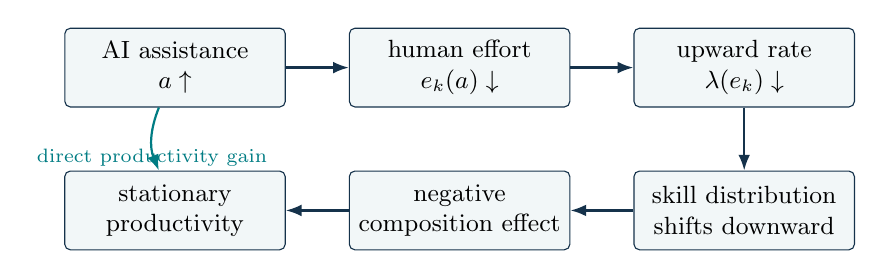
\begin{tikzpicture}[
  node distance=8mm,
  box/.style={draw=navy,rounded corners=2pt,fill=pale,minimum width=28mm,
    minimum height=10mm,align=center,font=\small},
  arr/.style={-{Latex[length=2mm]},thick,navy}]
\node[box] (a) {AI assistance\\$a\uparrow$};
\node[box,right=of a] (e) {human effort\\$e_k(a)\downarrow$};
\node[box,right=of e] (l) {upward rate\\$\lambda(e_k)\downarrow$};
\node[box,below=of l] (pi) {skill distribution\\shifts downward};
\node[box,left=of pi] (comp) {negative\\composition effect};
\node[box,left=of comp] (P) {stationary\\productivity};
\draw[arr] (a)--(e);
\draw[arr] (e)--(l);
\draw[arr] (l)--(pi);
\draw[arr] (pi)--(comp);
\draw[arr] (comp)--(P);
\draw[-{Latex[length=2mm]},thick,teal] (a) to[bend right=22]
  node[below,font=\scriptsize]{direct productivity gain} (P);
\end{tikzpicture}
\vspace{6mm}
\begin{block}{The theorem compares the two paths}
$\Delta_m$ measures their local relative sensitivities, while $\mu$ determines how strongly the learning path influences long-run weights.
\end{block}
\end{frame}

\begin{frame}{Final conclusions}
\begin{enumerate}
  \item \textbf{Static substitution is exact:}
  \[
  e^\star(s,a)=\pos{x^\star-s-a}.
  \]
  \item \textbf{Fixed-skill productivity never falls:}
  \[
  p^\star(s,a)=\max\{p(x^\star),p(s+a)\}.
  \]
  \item \textbf{Endogenous learning shifts stationary mass toward low skill.}
  \item \textbf{Within each activity regime, productivity has at most one interior peak.}
  \item \textbf{A positive sensitivity gap and sufficiently large decay create a declining region.}
  \item \textbf{The paradox is compositional, not a failure of the direct productivity effect.}
\end{enumerate}
\end{frame}

\begin{frame}{Questions that test real understanding}
\begin{enumerate}
  \item Why is $x^{\mathrm{opt}}=\max\{x^\star,s+a\}$ rather than a minimum?
  \item Why may a transition rate exceed one?
  \item Which normalization step produces the exponent $-1$ in $\pi_1(a)$?
  \item Why does $r_i^\ell\ge r_i^h$ imply a lower stationary lower tail?
  \item Which terms in $\calP'(a)$ are the direct gain and composition loss?
  \item Why does Cauchy--Schwarz imply at most one derivative crossing?
  \item What role does $\mu$ play beyond the sign of $\Delta_m$?
\end{enumerate}
\vspace{3mm}
\centering
\large A correct answer connects the algebra to the economic mechanism.
\end{frame}

\begin{frame}{References and scope}
\small
\begin{thebibliography}{9}
\bibitem{ALZ}
Ali Aouad, Thodoris Lykouris, and Huiying Zhong.
\newblock \emph{Human--AI Productivity Paradoxes: Modeling the Interplay of Skill, Effort, and AI Assistance}.
\newblock arXiv:2605.11350v1, 2026.

\bibitem{GS}
Geoffrey Grimmett and David Stirzaker.
\newblock \emph{Probability and Random Processes}, 3rd ed.
\newblock Oxford University Press, 2001.

\bibitem{Varian}
Hal R. Varian.
\newblock \emph{Microeconomic Analysis}, 3rd ed.
\newblock W. W. Norton, 1992.
\end{thebibliography}
\vspace{3mm}
\begin{block}{Deck scope}
Tutorial Sections 3 and 4 only. Unreliable AI, AI literacy, and convex-cost extensions are outside this deck.
\end{block}
\vfill
\centering
\href{mailto:aquisper@caltech.edu}{aquisper@caltech.edu}
\end{frame}

\end{document}
